\begin{center}
	\begin{tabular}{M{9.25cm}M{8.75cm}}
		\textbf{TRƯỜNG THCS-THPT NGUYỄN KHUYẾN}& \textbf{ÔN TẬP KTTX LẦN 1 - HỌC KÌ 2}\\
		\textbf{MÃ ĐỀ: 005}& \textbf{Bài thi môn: VẬT LÝ 10}\\
		\textit{(Đề thi có 04 trang)}& \textit{Thời gian làm bài: 40 phút, không kể phát đề}
		
		\noindent\rule{4cm}{0.8pt} \\
	\end{tabular}
\end{center}
\vspace{-0.5cm}
\setcounter{section}{0}
\section{Câu trắc nghiệm nhiều phương án lựa chọn}
\textit{Thí sinh trả lời từ câu 1 đến câu 12. Mỗi câu hỏi thí sinh chọn một phương án}
\setcounter{ex}{0}
\Opensolutionfile{ans}[ans/D10-KTTX3-001-TN]
% ===================================================================
\begin{ex}
\immini{Ba bình thủy tinh cùng đựng nước như hình bên, độ cao cột nước trong các bình là như nhau. Áp suất tại đáy bình nào là lớn nhất?
\choice
{Bình A}
{Bình B}
{Bình C}
{\True Áp suất tại đáy 3 bình như nhau}
}
{\includegraphics[scale=0.6]{../figs/D10-KTTX3-001-2}}
	\loigiai{}
\end{ex}
% ===================================================================
\begin{ex}
	Một vật có trục quay cố định, chịu tác dụng của lực $\vec{F}_1$ (với cánh tay đòn $d_1$) và lực $\vec{F}_2$ (với cánh tay đòn $d_2$). Vật cân bằng thì điều kiện cân bằng của vật là
	\choice
	{\True $F_1\cdot d_1=F_2\cdot d_2$}
	{$F_1\cdot d_2=F_2\cdot d_1$}
	{$F_1\cdot F_2=d_1\cdot d_2$}
	{$\left(F_1+F_2\right)\cdot\left(d_1+d_2\right)=0$}
	\loigiai{}
\end{ex}
% ===================================================================
\begin{ex}
	Các tàu ngầm thường được thiết kế giống với hình dạng cá heo để
	\choice
	{\True giảm thiểu lực cản}
	{đẹp mắt}
	{tiết kiệm chi phí chế tạo}
	{tăng thể tích khoang chứa}
	\loigiai{}
\end{ex}
% ===================================================================
\begin{ex}
	Chọn phát biểu đúng.
	\choice
	{Moment lực tác dụng lên vật là đại lượng vô hướng}
	{\True Moment lực đối với một trục quay được đo bằng tích của lực với cánh tay đòn của nó}
	{Moment lực là đại lượng đặc trưng cho độ mạnh yếu của lực}
	{Đơn vị của moment lực là $\si{\newton/\meter}$}
	\loigiai{}
\end{ex}
% ===================================================================
\begin{ex}
	Hình dạng nào của vật cho lực cản nhỏ nhất?
	\choice
	{Khối cầu}
	{\True Hình dạng khí động học}
	{Khối lập phương}
	{Khối trụ dài}
	\loigiai{}
\end{ex}
% ===================================================================
\begin{ex}
	\immini{Dùng kéo để cắt một sợi dây kim loại theo 3 trường hợp như hình bên. Chỉ xét thành phần lực vuông góc do 1 ngón tay tác dụng lên kéo như trên hình. 
		}
	{\includegraphics[scale=0.6]{../figs/D10-KTTX3-001-4}}
	So sánh độ lớn thành phần lực $F_\mathrm{A}$, $F_\mathrm{B}$ và $F_\mathrm{C}$ cần tác dụng vào kéo để cắt đứt dây (lực trên hình không đúng tỉ lệ độ lớn).
	\choice
	{$F_{\mathrm{C}}>F_{\mathrm{B}}>F_{\mathrm{A}}$}
	{\True $F_{\mathrm{A}}>F_{\mathrm{C}}>F_{\mathrm{B}}$}
	{$F_{\mathrm{B}}>F_{\mathrm{C}}>F_{\mathrm{A}}$}
	{$F_{\mathrm{A}}=F_{\mathrm{B}}=F_{\mathrm{C}}$}
	\loigiai{}
\end{ex}
% ===================================================================
\begin{ex}
	Chọn phát biểu đúng.
	\choice
	{Độ lớn lực cản càng lớn khi diện tích mặt cản càng nhỏ}
	{Độ lớn của lực cản không phụ thuộc vào tốc độ của vật}
	{Vật đi càng nhanh thì lực cản của không khí càng nhỏ}
	{\True Tờ giấy để phẳng rơi chậm hơn hòn đá khi cùng được thả từ trạng thái nghỉ trong không khí}
	\loigiai{}
\end{ex}

% ===================================================================
\begin{ex}
	Có ba bình như nhau đựng ba loại chất lỏng có cùng độ cao. Bình (1) đựng cồn, bình (2) đựng nước, bình (3) đựng nước muối. Gọi $p_1$, $p_2$, $p_3$ là áp suất khối chất lỏng tác dụng lên đáy các bình (1), (2), (3). Điều nào dưới đây là đúng?
	\choice
	{$p_1>p_2>p_3$}
	{$p_2>p_1>p_3$}
	{\True $p_3>p_2>p_1$}
	{$p_2>p_3>p_1$}
	\loigiai{}
\end{ex}
% ===================================================================
\begin{ex}
\immini{	Biết các lực $F_1=\SI{25}{\newton}$, $F_2=\SI{10}{\newton}$, $F_3=\SI{10}{\newton}$ tác dụng vào thanh AB như hình vẽ. Quy ước moment của các lực làm thanh AB quay ngược chiều kim đồng hồ mang giá trị dương. Moment của các lực $\vec{F}_1$, $\vec{F}_2$, $\vec{F}_3$ đối với trục quay qua A lần lượt là
\choice
{\SI{-8}{\newton\cdot\meter}; \SI{8.5}{\newton\cdot\meter}; \SI{0}{\newton\cdot\meter}}
{\SI{-0.8}{\newton\cdot\meter}; \SI{8.5}{\newton\cdot\meter}; \SI{0}{\newton\cdot\meter}}
{\SI{8}{\newton\cdot\meter}; \SI{8.5}{\newton\cdot\meter}; \SI{0}{\newton\cdot\meter}}
{\True \SI{8.5}{\newton\cdot\meter}; \SI{-8}{\newton\cdot\meter}; \SI{0}{\newton\cdot\meter}}
}
{	\begin{tikzpicture}
			\coordinate (B) at (0,0);
			\coordinate (A)  at ($(B)+(200:4)$);
			\coordinate (F1)  at ($(B)+(175:2.5)$);
			\coordinate (F3)  at ($(B)+(20:2)$);
			\coordinate (F2)  at ($(B)+(-70:2)$);
			\coordinate (C)  at ($(B)+(175:3.625)$);
			\tkzMarkRightAngle[size=0.3,color=red, line width=1pt](A,B,F2);
			\tkzMarkRightAngle[size=0.3, line width=1pt](A,C,B);
			\draw[line width=3pt] (A)--(B);
			\draw[dashed, line width=1pt] (A)--(C)--(B);
			\draw[blue, line width=2pt, -stealth] (B)--(F1);
			\draw[blue, line width=2pt, -stealth] (B)--(F2);
			\draw[blue, line width=2pt, -stealth] (B)--(F3);
			\fill   (A) circle[radius=4pt]  node [below left] {A};
			\node[above, blue] at (F1) {$\vec{F_1}$};
			\node[above, blue] at (F3) {$\vec{F_3}$};
			\node[right, blue] at (F2) {$\vec{F_2}$};
			\node[above] at (B) {B};
			\node[above] at (C) {C};
			\node[below] at ($(A)!0.5!(B)-(0,0.25)$) {$\SI{80}{\centi\meter}$};
			\tkzMarkAngle[size=0.75cm,color=red, line width=1pt](F1,B,A);
			\tkzLabelAngle[color=black,pos=1.2](F1,B,A){$\SI{25}{\degree}$};
			
		\end{tikzpicture}
}
	\loigiai{}
\end{ex}
% ===================================================================
\begin{ex}
	Một thanh AB dài $\SI{7.5}{\meter}$ có trọng lượng $\SI{200}{\newton}$ và trọng tâm G cách đầu A một đoạn $\SI{2}{\meter}$. Thanh có thể quay xung quanh một trục đi qua O. Biết $\mathrm{OA}=\SI{2.5}{\meter}$. Phải tác dụng vào đầu B một lực $\vec{F}$ có độ lớn bằng bao nhiêu để AB cân bằng?
	\choice
	{\SI{100}{\newton}}
	{\SI{25}{\newton}}
	{\SI{10}{\newton}}
	{\True \SI{20}{\newton}}
	\loigiai{}
\end{ex}
% ===================================================================
\begin{ex}
	\immini{Đĩa phẳng có thể quay quanh trục quay $\Delta$ như hình bên. Tác dụng  lực $\vec{F}$ có độ lớn $\SI{10}{\newton}$ tại điểm cách trục quay $\SI{12}{\centi\meter}$. Giá của $\vec{F}$ hợp với mặt đĩa góc $\SI{60}{\degree}$. Moment do lực $\vec{F}$ gây ra đối với trục quay $\Delta$ là \choice
		{\SI{1.2}{\newton\cdot\meter}}
		{\SI{1.04}{\newton\cdot\meter}}
		{\True \SI{0.6}{\newton\cdot\meter}}
		{\SI{0.83}{\newton\cdot\meter}}}
	{\vspace{-0.75cm}\includegraphics[scale=0.2]{../figs/D10-KTTX3-001-6}}
	
	\loigiai{}
\end{ex}
% ===================================================================
\begin{ex}
\immini{	Một thanh AB đồng chất, tiết diện đều có khối lượng $\SI{3}{\kilogram}$, dài $\SI{2}{\meter}$, có một đầu được gắn bởi một bản lề nhẵn vào trần nhà tại A. Đầu B được buộc vào một sợi dây nhẹ không đàn hồi. Đầu kia của sợi dây được gắn vào trần nhà ở điểm C. Thanh tạo một góc $\SI{30}{\degree}$ với phương ngang và sợi dây tạo một góc $\SI{60}{\degree}$ so với phương ngang như hình bên. 	}
	{\begin{tikzpicture}
			\coordinate (A) at (0,0);
			\coordinate (B) at ($(A)+(-30:4)$);
			\coordinate (C) at (5,0);
			\tkzMarkAngle[size=0.75cm,color=blue,line width=1.5pt](B,A,C);
			\tkzLabelAngle[color=black,pos=1.2](B,A,C){$\SI{30}{\degree}$};
			\tkzMarkAngle[size=0.75cm,color=blue,line width=1.5pt](A,C,B);
			\tkzMarkAngle[size=0.65cm,color=blue,line width=1.5pt](A,C,B);
			\tkzLabelAngle[color=black,pos=1.2](A,C,B){$\SI{60}{\degree}$};
			
			\draw[line width=1pt, gray] (C)--(B);
			\draw[line width=6pt, gray] (-0.5,0)--(5.5,0);
			\node[above] at (A) {A};
			\node[above] at (C) {C};
			\node[below] at (B) {B};
			\draw[line width=3pt] (A)--(B);
			\filldraw[black] (A) circle(4pt);
	\end{tikzpicture}}
Lấy $g=\SI{10}{\meter/\second^2}$. Lực căng của sợi dây có độ lớn là
\choice
{$\SI{7.5}{\newton}$}
{$\SI{14}{\newton}$}
{\True $\SI{13}{\newton}$}
{$\SI{6.5}{\newton}$}
	\loigiai{}
\end{ex}
\Closesolutionfile{ans}
\section{Câu trắc nghiệm đúng/sai} 
\textit{Thí sinh trả lời từ câu 1 đến câu 4. Trong mỗi ý \textbf{a)}, \textbf{b)}, \textbf{c)}, \textbf{d)} ở mỗi câu, thí sinh chọn đúng hoặc sai}
\setcounter{ex}{0}\\
\Opensolutionfile{ans}[ans/D10-KTTX3-001-TF]
% ===================================================================
\begin{ex} Trong các phát biểu sau, phát biểu nào đúng, phát biểu nào sai?
	\choiceTF
	{Ngẫu lực là hệ gồm hai lực song song, ngược chiều và có độ lớn bằng nhau. Do đó, hợp lực của ngẫu lực bằng không}
	{\True Nếu vật không có trục quay cố định chịu tác dụng của ngẫu lực thì nó sẽ quay quanh một trục đi qua trọng tâm và vuông góc với mặt phẳng chứa ngẫu lực}
	{\True Moment của ngẫu lực tính theo công thức: $M=F\cdot d$ (trong đó $d$ là khoảng cách giữa giá của hai lực thành phần)}
	{Khi tác dụng một lực $\vec{F}$ có giá đi qua trọng tâm của một vật thì vật đó sẽ vừa chuyển động tịnh tiến vừa chuyển động quay}
	\loigiai{}
\end{ex}
% ===================================================================
\begin{ex}
	Hai anh em Bình và An đang chơi trò bập bênh. Bập bênh là một tấm ván AB cứng, đồng chất, tiết diện đều và giá đỡ nằm ngay trọng tâm O của tấm ván. AB chia thành 6 đoạn bằng nhau (như hình). Khối lượng của An bằng $\SI{25}{\kilogram}$ còn khối lượng của Bình bằng $\SI{75}{\kilogram}$. An ngồi bên phần OA và Bình ngồi bên phần OB.
	\begin{center}
		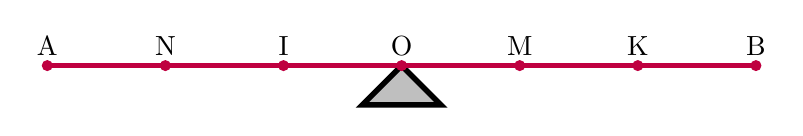
\begin{tikzpicture}
			\draw[line width=2pt, fill=gray!50!white] (0,0)--(-0.5,-0.5)--(0.5,-0.5)--(0,0);
			\draw[line width=2pt, purple] (-4.5,0)--(4.5,0);
			\foreach \i in {-4.5,-3,...,4.5}{
				\fill[fill=purple]   (\i,0) circle[radius=2pt];
				
			};
			\node[above] at (-4.5,0) {A};
			\node[above] at (-1.5,0) {I};
			\node[above] at (-3,0) {N};
			\node[above] at (0,0) {O};
			\node[above] at (1.5,0) {M};
			\node[above] at (3,0) {K};
			\node[above] at (4.5,0) {B};
		\end{tikzpicture}
	\end{center}
	\choiceTF
	{\True Bập bênh trên không có moment trọng lực}
	{Khi Bình và An cùng ngồi tại hai đầu tấm ván thì moment trọng lực của hai anh em bằng nhau }
	{Khi Bình và An cùng ngồi tại hai đầu tấm ván thì bập bênh có xu hướng quay ngược chiều kim đồng hồ}
	{\True Khi An ngồi ở A, để bập bênh ở trạng thái cân bằng nằm ngang thì Bình phải dịch chuyển tới vị trí M}
	\loigiai{
		\begin{itemchoice}
			\itemch Đúng.
			\itemch Sai. Do $\mathrm{OA}=\mathrm{OB}$ và $m_{\text{Bình}}>m_{\text{An}}$ nên $M_{\vec{P}\text{An}}<M_{\vec{P}{\text{Bình}}}$.
			\itemch Sai. Do $M_{\vec{P}\text{An}}<M_{\vec{P}\text{Bình}}$ nên bập bênh có xu hướng quay cùng chiều kim đồng hồ.
			\itemch Đúng.
		\end{itemchoice}
	}
\end{ex}
% ===================================================================
\begin{ex}
	Một bình trụ đế nằm ngang diện tích $\SI{50}{\centi\meter^2}$ chứa 1 lít nước, biết khối lượng riêng của nước là $\rho_{\mathrm{n}}=\SI{1000}{\kilogram/\meter^3}$. Lấy $g=\SI{9.8}{\meter/\second^2}$. Áp suất khí quyển $p_0=\SI{1.013E5}{\pascal}$, gia tốc trọng trường $g=\SI{9.8}{\meter/\second^2}$.
	\choiceTF
	{\True Chiều cao của nước trong bình là $\SI{20}{\centi\meter}$}
	{\True Độ chênh lệch áp suất giữa đáy bình và mặt thoáng của nước là $\SI{1960}{\pascal}$}
	{\True Áp suất ở đáy bình xấp xỉ bằng $\SI{1.033E5}{\pascal}$}
	{Người ta đặt lên mặt thoáng của nước một piston có khối lượng $\SI{2}{\kilogram}$, đường kính bằng đường kính trong của bình. Coi piston có thể trượt không ma sát lên thành bình. Áp suất tác dụng lên đáy bình là $\SI{2E5}{\pascal}$}
	\loigiai{}
\end{ex}
% ===================================================================
\begin{ex}
	\immini{Khi một viên bi hình cầu chuyển động trong chất lỏng, viên bi chịu tác dụng của lực cản được gọi là lực nội ma sát. Biểu thức độ lớn của lực nội ma sát được xác định bởi định luật Stokes: $f=6\pi\eta r v$, trong đó:
	\begin{itemize}
		\item $f$ là lực nội ma sát;
		\item $r$ là bán kính viên bi;
		\item $v$ tốc độ tức thời của viên bi;
		\item $\eta$ là hệ số ma sát nhớt hay độ nhớt của chất lỏng.
	\end{itemize}	
	}
	{\vspace{-0.75cm}\includegraphics[scale=0.5]{../figs/D10-KTTX3-001-8}}
	Độ lớn lực nội ma sát tăng tỉ lệ thuận với tốc độ của viên bi, khi lực đẩy Archimedes và lực nội ma sát triệt tiêu hoàn toàn trọng lực của bi thì viên bi sẽ chuyển động đều với tốc độ giới hạn $v_{\mathrm{gh}}$. Hình bên là sơ đồ bố trí thí nghiệm định luật Stokes. Tốc độ giới hạn của viên bi có thể được xác định thông qua thời gian chuyển động $t$ của viên bi rơi thẳng đều giữa hai vị trí cổng quang cách nhau khoảng $L$.\\
	Một nhóm học sinh thực hiện thí nghiệm xác định hệ số ma sát nhớt của dầu với các số liệu cố định và bảng kết quả thời gian rơi như sau:
	\begin{itemize}
		\item Khối lượng riêng của dầu: $\rho=\xsi{900\pm10}{\kilogram/\meter^3}$;
		\item Khối lượng riêng của viên bi: $\sigma=\xsi{7890\pm 10}{\kilogram/\meter^3}$;
		\item Gia tốc trọng trường: $g=\xsi{9,81\pm 0,01}{\meter/\second^2}$;
		\item Khoảng cách 2 cổng quang: $L=\xsi{30,0\pm 0,1}{\centi\meter}$;
		\item Đường kính viên bi: $d=\xsi{6,84\pm0,02}{\milli\meter}$.
	\end{itemize}
	
	\begin{center}
		\textbf{Bảng kết quả thời gian bi rơi giữa hai cổng quang}\\
		\begin{tabular}{|M{4cm}|M{2cm}|M{2cm}|M{2cm}|M{2cm}|M{2cm}|}
			\hline
			\thead{Lần đo} & 1& 2 & 3 & 4 & 5 \\
			\hline
			\thead{Thời gian $\left(\si{\second}\right)$} & $\SI{0.579}{}$ & $\SI{0.579}{}$ & $\SI{0.578}{}$ & $\SI{0.577}{}$ & $\SI{0.579}{}$\\
			\hline
		\end{tabular}
	\end{center}
	Xem đường kính viên bi là rất nhỏ so với đường kính ống thủy tinh.\\
	\textit{Gợi ý: Thể tích hình cầu bán kính $r$ được xác định bởi $V=\dfrac{4}{3}\pi r^3$.}
	\choiceTF
	{Đồng hồ đo thời gian hiện số được đặt ở mode A + B}
	{\True Tốc độ giới hạn của viên bi xấp xỉ $\SI{51.9}{\centi\meter/\second}$}
	{Độ lớn lực nội ma sát tác dụng lên viên bi đang chuyển động ở tốc độ giới hạn là $\SI{0.013}{\newton}$}
	{\True Hệ số ma sát nhớt đo được trong điều kiện thí nghiệm trên là $\SI{0.34}{\kilogram\cdot\meter^{-1}\cdot\second^{-1}}$}

	\loigiai{}
\end{ex}
\Closesolutionfile{ans}
\section{Tự luận}
\setcounter{ex}{0}
\Opensolutionfile{ans}[ans/D10-KTTX3-001-TL]
% ======================================================================
\begin{ex}\textit{(1,0 điểm)} 
	Vì sao chân đập nước luôn được thiết kế dày hơn đỉnh đập nước?
	\begin{center}
		\includegraphics[scale=0.4]{../figs/D10-KTTX3-001-5}
	\end{center}
	\loigiai{}
\end{ex}
% ======================================================================
\begin{ex}\textit{(1,0 điểm)} 
	Hình dưới đây là thiết kế một chiếc bẫy chuột đơn giản, gồm:
	\begin{itemize}
		\item Thanh nhẹ có khối lượng không đáng kể so với con chuột và vật nặng, có thể quay quanh trục đi qua O. Trục quay được giữ cố định bởi giá đỡ gắn với cái xô.
		\item Vật nặng gắn với một đầu thanh nhẹ, điểm đặt trọng lực tại B.
		\item Chuột khi đi đến vị trí A thì bẫy sập xuống.
	\end{itemize}
	\begin{center}
		\includegraphics[scale=0.5]{../figs/D10-KTTX3-001-3}
	\end{center}
	\begin{enumerate}[label=\alph*)]
		\item Ban đầu, thiết kế được dùng để bắt chuột nâu. Biết khối lượng trung bình của chuột nâu là $m=\SI{300}{\gram}$, các kích thước $d_1=\SI{20}{\centi\meter}$; $d_2=\SI{5}{\centi\meter}$. Tính khối lượng vật nặng cần dùng.
		\item 	Ngoài chuột nâu, ở khu vực đặt bẫy có xuất hiện chuột đen. Chuột đen nặng trung bình $m'=\SI{150}{\gram}$ nên không sập bẫy. Phải làm đầu OA dài bao nhiêu để khi chỉ có một con chuột đen đến vị trí A thì bẫy vẫn sập xuống?
	\end{enumerate}
	\loigiai{}
\end{ex}
% ======================================================================
\begin{ex}\textit{(1,0 điểm)}
	Người ta đổ thêm $\SI{100}{\centi\meter^3}$ nước vào một nhánh của một bình hình chữ U có hai nhánh giống nhau đang chứa thủy ngân. Hỏi mặt thoáng của thủy ngân ở nhánh bên kia của bình di chuyển bao nhiêu $\si{\centi\meter}$? Biết đường kính trong của bình $d=\SI{2}{\centi\meter}$, khối lượng riêng của thủy ngân $\rho_{\ce{Hg}}=\SI{13600}{\kilogram/\meter^3}$ và của nước $\rho_{\ce{H_2O}}=\SI{1000}{\kilogram/\meter^3}$.
	\loigiai{$\SI{1.17}{\centi\meter}$}
\end{ex}
\Closesolutionfile{ans}
\begin{center}
	\textbf{--- HẾT ---}
\end{center}